\chapter{Comparación con Eventos de Dijets}\label{dijets}

Dentro del grupo de Física Experimental de Altas Energías del DF\footnote{Departamento de Física, FCEyN, UBA}, actualmente se está realizando un trabajo similar en torno a calibraciones R-scan, pero utilizando una selección de eventos de dijets.

Una vez realizada la selección de eventos correspondiente, se aplica el mismo método de direct-matching como fue explicado en la sección \ref{Rscan}. La ventaja de esta selección de eventos es que permite obtener una calibración al momento de Rscan Jets en un rango de momento más extendido, por ejemplo, alcanzando un momento de $p_t\sim$1TeV con una incerteza estadística del orden del 0.2$\%$ en los bines de $\eta$ centrales. Sin embargo, ésta no permite ir hacia valores de momento bajo: por debajo de $p_t<$100GeV la incerteza estadística asociada aumenta hasta el 1$\%$, y hasta el 2$\%$ por debajo de los 60GeV. Si bien este trabajo actualmente continúa en curso, en la figura \ref{fig:Comparison} se pueden ver resultados preliminares de dicho estudio con eventos de dijets para el caso de Rscan Jets con $R=$0.6. La incerteza sistemática que se muestra en la figura se corresponde a contribuciones de los parámetros del método de direct-matching: JVT, aislación ($f$) y matching ($dR$) (ver tabla \ref{tab:sel}) tomando los mismos valores para sus respectivas variaciones; y a la contribución de la elección del generador de MC. A esta incerteza sistemática, se le incorporó además la incerteza asociada a la JES, que es la misma que la aplicada en el caso de eventos de $Z+jets$. 

En la figura \ref{fig:Comparison} también se muestra la calibración derivada en esta tesis, junto con su incerteza total con el fin de comparar las calibraciones en el rango de momento en el que se solapan. De estas figuras queda claro como se distribuye la estadística para una selección de eventos y para la otra. Mientras que para el caso de $Z$+$jets$ se logra derivar una corrección para $p_t>$25GeV con una banda de error estadístico de ancho $<$1$\%$ hasta un $p_t\sim$100GeV, y aumentando  hasta un ancho de $\sim1$.5$\%$ en $p_t\sim300$GeV; para el caso de dijets se observa un comportamiento opuesto, con una componente estadística, en general, de ancho $>2\%$ y en algunos casos, como el de la figura \ref{fig:stat}, de ancho mayor al 8$\%$ a bajo momento, que disminuye hasta una ancho de 0.5$\%$ llegando a 1TeV. 

Ambas calibraciones comparten el rango de momento entre 45Gev$<p_t<$300GeV. En las figuras (a), (b) y (c) puede verse que en un primer tramo de este intervalo las bandas estadísticas de ambas calibraciones se solapan, mientras que en el resto del intervalo se observa que la superposición se da gracias a la contribución de las incertezas sistemáticas a la incerteza total. 

Si bien ambas selecciones de eventos se usan para derivar una calibración en dos rangos distintos pero que se superponen, no necesariamente debiera una ser, en algún sentido, ``continuación'' de la otra. Esta sospecha se encuentra relacionada con el hecho de que la selección de eventos de dijets, discrimina eventos de naturaleza QCD mientras que la de $Z$+$jets$ prioriza eventos de tipo semi-leptónicos.



\begin{figure}[ht]
    \centering
    \begin{subfigure}[b]{0.495\textwidth}
        \centering
        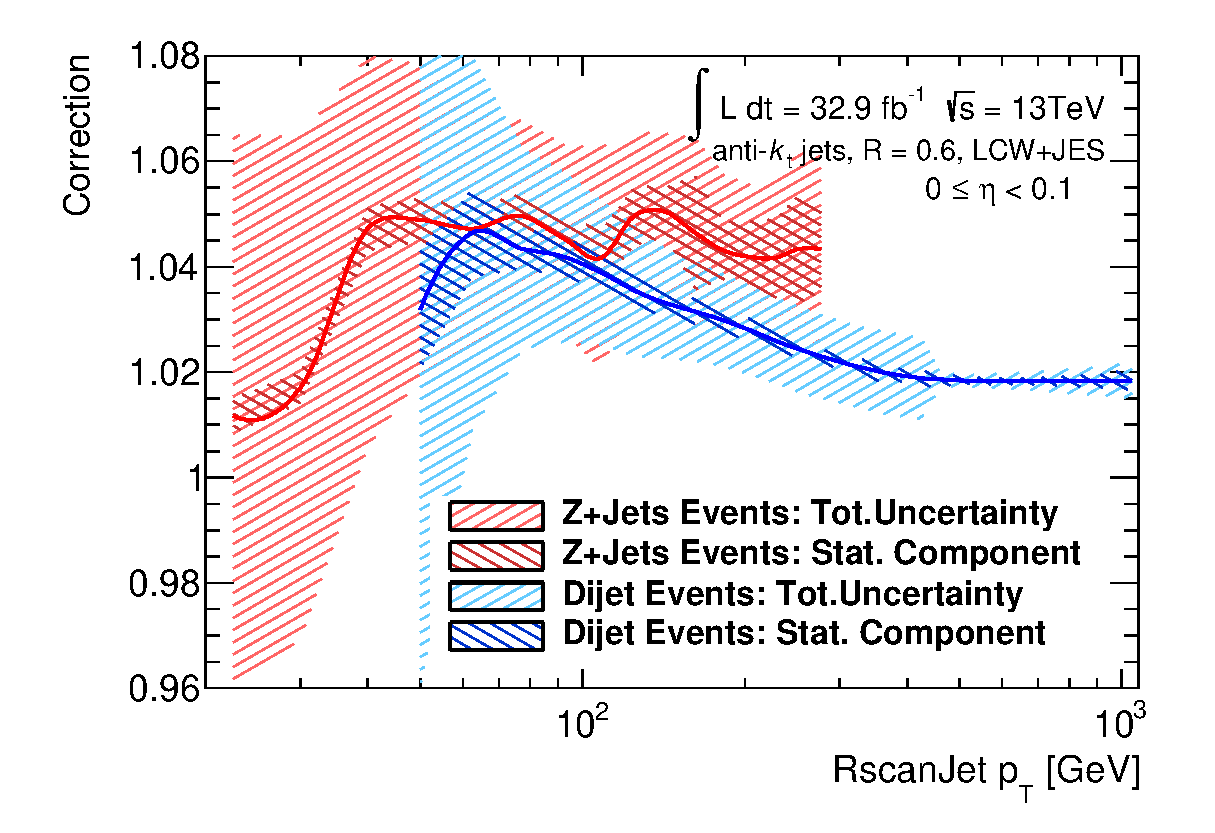
\includegraphics[width=\textwidth]{images/ComparisonW_dijets_Eta_45.eps}
        \caption{0.0$<\eta^{Rscan}_{det}<$0.1}
        %\label{fig:data2lc49}
    \end{subfigure}
    \hfill
    \begin{subfigure}[b]{0.495\textwidth}
        \centering
        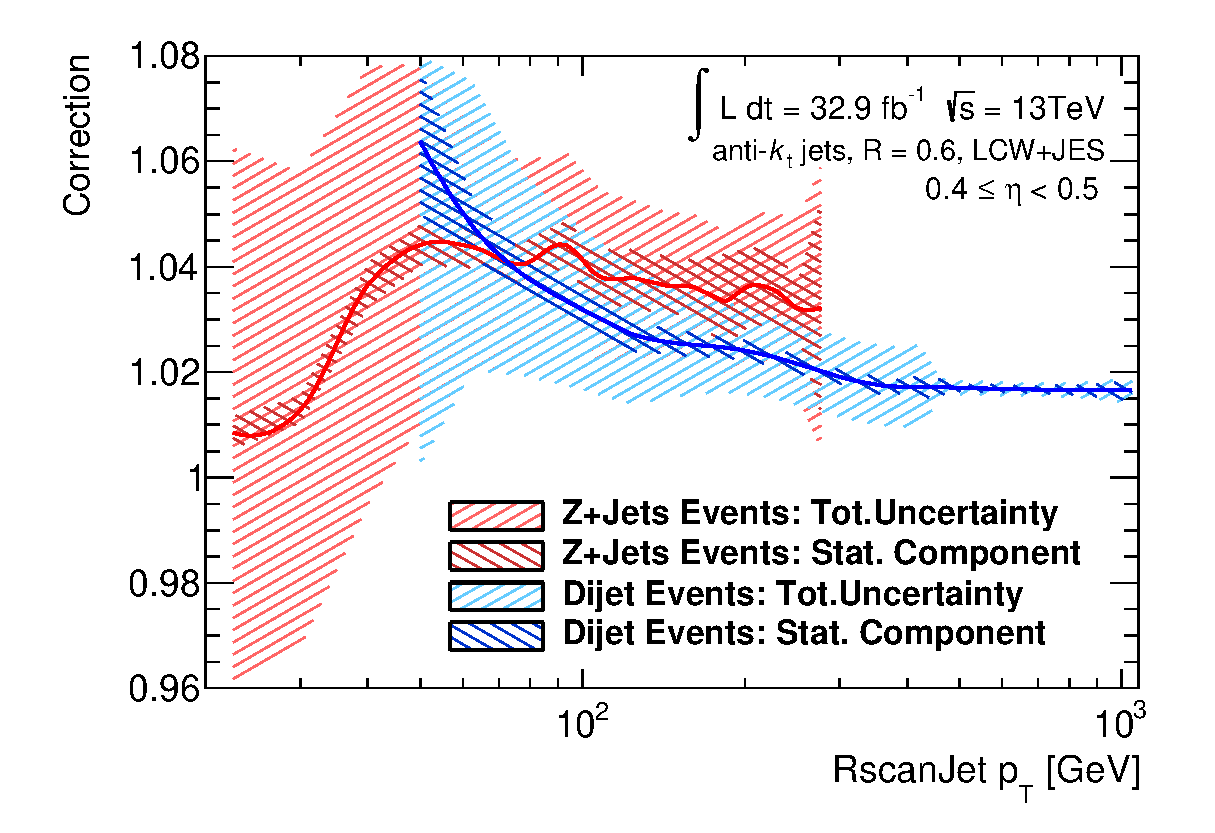
\includegraphics[width=\textwidth]{images/ComparisonW_dijets_Eta_49.eps}
        \caption{ 0.4$<\eta^{Rscan}_{det}<$0.5}
        %\label{fig:Th26lc}
    \end{subfigure}
    \vfill
    \begin{subfigure}[b]{0.495\textwidth}
        \centering
        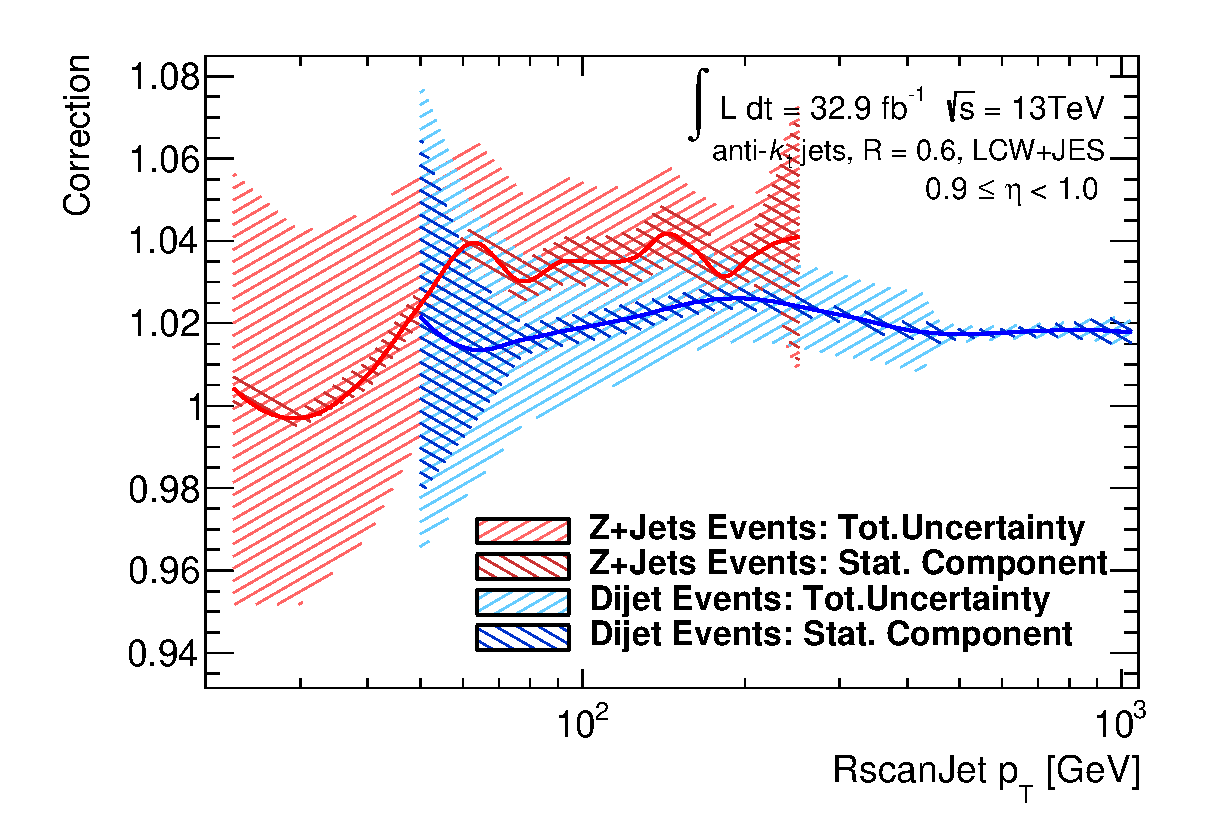
\includegraphics[width=\textwidth]{images/ComparisonW_dijets_Eta_54.eps}
        \caption{0.9$<\eta^{Rscan}_{det}<$1.0}
        \label{fig:stat}
    \end{subfigure}
    \hfill
    \begin{subfigure}[b]{0.495\textwidth}
        \centering
        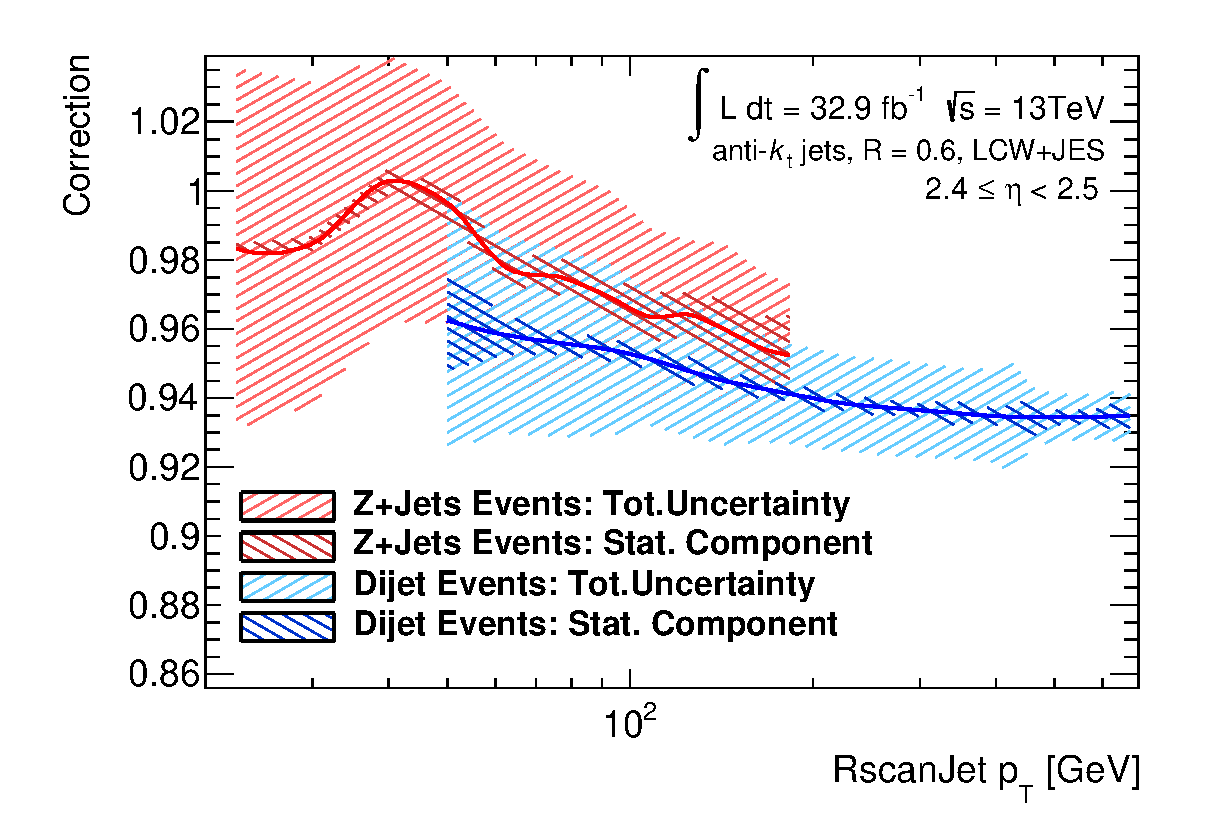
\includegraphics[width=\textwidth]{images/ComparisonW_dijets_Eta_69.eps}
        \caption{2.4$<\eta^{Rscan}_{det}<$2.5}
        %\label{fig:Th26lc}
    \end{subfigure}
    \caption{ Comparación entre la calibración Rscan derivada para Rscan Jets de radio 0.6 en eventos de $Z+jets$ (en rojo) y en eventos de dijets (en azul) para distintos bines de $\eta$. Para cada calibración se muestra también la incerteza total y su componente estadística.} 
    \label{fig:Comparison}
\end{figure}









